

\tikzset{every picture/.style={line width=0.75pt}} %set default line width to 0.75pt        

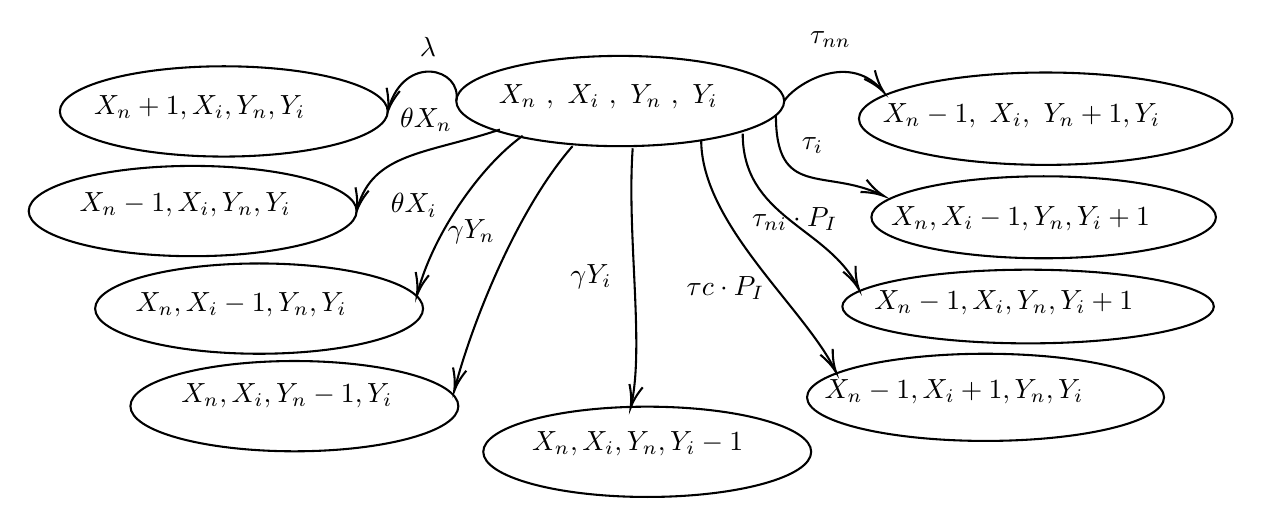
\begin{tikzpicture}[x=0.75pt,y=0.75pt,yscale=-1,xscale=1]
%uncomment if require: \path (0,300); %set diagram left start at 0, and has height of 300

%Shape: Ellipse [id:dp7831011517338047] 
\draw   (240,74.75) .. controls (240,62.74) and (275.37,53) .. (319,53) .. controls (362.63,53) and (398,62.74) .. (398,74.75) .. controls (398,86.76) and (362.63,96.5) .. (319,96.5) .. controls (275.37,96.5) and (240,86.76) .. (240,74.75) -- cycle ;
%Shape: Ellipse [id:dp462622419782051] 
\draw   (49,79.75) .. controls (49,67.74) and (84.37,58) .. (128,58) .. controls (171.63,58) and (207,67.74) .. (207,79.75) .. controls (207,91.76) and (171.63,101.5) .. (128,101.5) .. controls (84.37,101.5) and (49,91.76) .. (49,79.75) -- cycle ;
%Shape: Ellipse [id:dp256860971375783] 
\draw   (34,127.75) .. controls (34,115.74) and (69.37,106) .. (113,106) .. controls (156.63,106) and (192,115.74) .. (192,127.75) .. controls (192,139.76) and (156.63,149.5) .. (113,149.5) .. controls (69.37,149.5) and (34,139.76) .. (34,127.75) -- cycle ;
%Shape: Ellipse [id:dp566194612238101] 
\draw   (66,174.75) .. controls (66,162.74) and (101.37,153) .. (145,153) .. controls (188.63,153) and (224,162.74) .. (224,174.75) .. controls (224,186.76) and (188.63,196.5) .. (145,196.5) .. controls (101.37,196.5) and (66,186.76) .. (66,174.75) -- cycle ;
%Shape: Ellipse [id:dp007245637900635815] 
\draw   (83,221.75) .. controls (83,209.74) and (118.37,200) .. (162,200) .. controls (205.63,200) and (241,209.74) .. (241,221.75) .. controls (241,233.76) and (205.63,243.5) .. (162,243.5) .. controls (118.37,243.5) and (83,233.76) .. (83,221.75) -- cycle ;
%Shape: Ellipse [id:dp07068175225961304] 
\draw   (253,243.75) .. controls (253,231.74) and (288.37,222) .. (332,222) .. controls (375.63,222) and (411,231.74) .. (411,243.75) .. controls (411,255.76) and (375.63,265.5) .. (332,265.5) .. controls (288.37,265.5) and (253,255.76) .. (253,243.75) -- cycle ;
%Shape: Ellipse [id:dp6329768531871176] 
\draw   (434,83.25) .. controls (434,70.96) and (474.29,61) .. (524,61) .. controls (573.71,61) and (614,70.96) .. (614,83.25) .. controls (614,95.54) and (573.71,105.5) .. (524,105.5) .. controls (474.29,105.5) and (434,95.54) .. (434,83.25) -- cycle ;
%Shape: Ellipse [id:dp9330369675466057] 
\draw   (440,130.75) .. controls (440,119.84) and (477.16,111) .. (523,111) .. controls (568.84,111) and (606,119.84) .. (606,130.75) .. controls (606,141.66) and (568.84,150.5) .. (523,150.5) .. controls (477.16,150.5) and (440,141.66) .. (440,130.75) -- cycle ;
%Shape: Ellipse [id:dp42671538978966184] 
\draw   (426,173.75) .. controls (426,163.95) and (466.07,156) .. (515.5,156) .. controls (564.93,156) and (605,163.95) .. (605,173.75) .. controls (605,183.55) and (564.93,191.5) .. (515.5,191.5) .. controls (466.07,191.5) and (426,183.55) .. (426,173.75) -- cycle ;
%Shape: Ellipse [id:dp8450878093450997] 
\draw   (409,217.5) .. controls (409,205.9) and (447.5,196.5) .. (495,196.5) .. controls (542.5,196.5) and (581,205.9) .. (581,217.5) .. controls (581,229.1) and (542.5,238.5) .. (495,238.5) .. controls (447.5,238.5) and (409,229.1) .. (409,217.5) -- cycle ;
%Curve Lines [id:da5430016808257252] 
\draw    (240,74.75) .. controls (242.94,58.82) and (215.15,51.78) .. (207.45,78.1) ;
\draw [shift={(207,79.75)}, rotate = 283.92] [color={rgb, 255:red, 0; green, 0; blue, 0 }  ][line width=0.75]    (10.93,-3.29) .. controls (6.95,-1.4) and (3.31,-0.3) .. (0,0) .. controls (3.31,0.3) and (6.95,1.4) .. (10.93,3.29)   ;
%Curve Lines [id:da8315854704549415] 
\draw    (261,88.5) .. controls (225.72,100.26) and (200.04,99.53) .. (192.44,126.09) ;
\draw [shift={(192,127.75)}, rotate = 283.92] [color={rgb, 255:red, 0; green, 0; blue, 0 }  ][line width=0.75]    (10.93,-3.29) .. controls (6.95,-1.4) and (3.31,-0.3) .. (0,0) .. controls (3.31,0.3) and (6.95,1.4) .. (10.93,3.29)   ;
%Curve Lines [id:da42020752488035984] 
\draw    (272,91.5) .. controls (251.42,106.2) and (228.92,138.91) .. (221.44,166.8) ;
\draw [shift={(221,168.5)}, rotate = 283.92] [color={rgb, 255:red, 0; green, 0; blue, 0 }  ][line width=0.75]    (10.93,-3.29) .. controls (6.95,-1.4) and (3.31,-0.3) .. (0,0) .. controls (3.31,0.3) and (6.95,1.4) .. (10.93,3.29)   ;
%Curve Lines [id:da7386528264768568] 
\draw    (296,96.5) .. controls (268.56,127.86) and (246.88,183.95) .. (239.44,212.77) ;
\draw [shift={(239,214.5)}, rotate = 283.92] [color={rgb, 255:red, 0; green, 0; blue, 0 }  ][line width=0.75]    (10.93,-3.29) .. controls (6.95,-1.4) and (3.31,-0.3) .. (0,0) .. controls (3.31,0.3) and (6.95,1.4) .. (10.93,3.29)   ;
%Curve Lines [id:da22159988103434247] 
\draw    (325,97.5) .. controls (322.06,138.66) and (330.64,192.07) .. (324.4,220.77) ;
\draw [shift={(324,222.5)}, rotate = 283.92] [color={rgb, 255:red, 0; green, 0; blue, 0 }  ][line width=0.75]    (10.93,-3.29) .. controls (6.95,-1.4) and (3.31,-0.3) .. (0,0) .. controls (3.31,0.3) and (6.95,1.4) .. (10.93,3.29)   ;
%Curve Lines [id:da4828436161819216] 
\draw    (358,93.5) .. controls (358,133.89) and (407.48,174.27) .. (422.35,204.14) ;
\draw [shift={(423,205.5)}, rotate = 244.98000000000002] [color={rgb, 255:red, 0; green, 0; blue, 0 }  ][line width=0.75]    (10.93,-3.29) .. controls (6.95,-1.4) and (3.31,-0.3) .. (0,0) .. controls (3.31,0.3) and (6.95,1.4) .. (10.93,3.29)   ;
%Curve Lines [id:da24512952467473603] 
\draw    (378,90.5) .. controls (378,130.68) and (418.34,135.33) .. (433.13,163.73) ;
\draw [shift={(434,165.5)}, rotate = 244.98000000000002] [color={rgb, 255:red, 0; green, 0; blue, 0 }  ][line width=0.75]    (10.93,-3.29) .. controls (6.95,-1.4) and (3.31,-0.3) .. (0,0) .. controls (3.31,0.3) and (6.95,1.4) .. (10.93,3.29)   ;
%Curve Lines [id:da7883161961005447] 
\draw    (394,81.5) .. controls (394,121.68) and (417.05,107.12) .. (444.32,119.7) ;
\draw [shift={(446,120.5)}, rotate = 206.57] [color={rgb, 255:red, 0; green, 0; blue, 0 }  ][line width=0.75]    (10.93,-3.29) .. controls (6.95,-1.4) and (3.31,-0.3) .. (0,0) .. controls (3.31,0.3) and (6.95,1.4) .. (10.93,3.29)   ;
%Curve Lines [id:da8370134985473645] 
\draw    (398,74.75) .. controls (401.9,67.93) and (427.66,50.41) .. (444.71,69) ;
\draw [shift={(446,70.5)}, rotate = 231.01] [color={rgb, 255:red, 0; green, 0; blue, 0 }  ][line width=0.75]    (10.93,-3.29) .. controls (6.95,-1.4) and (3.31,-0.3) .. (0,0) .. controls (3.31,0.3) and (6.95,1.4) .. (10.93,3.29)   ;

% Text Node
\draw (259,65.4) node [anchor=north west][inner sep=0.75pt]    {$X_{n} \ ,\ X_{i} \ ,\ Y_{n} \ ,\ Y_{i} \ $};
% Text Node
\draw (444,74.4) node [anchor=north west][inner sep=0.75pt]    {$X_{n} -1,\ X_{i} ,\ Y_{n} +1,Y_{i}$};
% Text Node
\draw (448,123.9) node [anchor=north west][inner sep=0.75pt]    {$X_{n} ,X_{i} -1,Y_{n} ,Y_{i} +1$};
% Text Node
\draw (440,164.4) node [anchor=north west][inner sep=0.75pt]    {$X_{n} -1,X_{i} ,Y_{n} ,Y_{i} +1$};
% Text Node
\draw (64,70.4) node [anchor=north west][inner sep=0.75pt]    {$X_{n} +1,X_{i} ,Y_{n} ,Y_{i}$};
% Text Node
\draw (416,207.4) node [anchor=north west][inner sep=0.75pt]    {$X_{n} -1,X_{i} +1,Y_{n} ,Y_{i}$};
% Text Node
\draw (275,232.4) node [anchor=north west][inner sep=0.75pt]    {$X_{n} ,X_{i} ,Y_{n} ,Y_{i} -1$};
% Text Node
\draw (106,209.4) node [anchor=north west][inner sep=0.75pt]    {$X_{n} ,X_{i} ,Y_{n} -1,Y_{i}$};
% Text Node
\draw (84,165.4) node [anchor=north west][inner sep=0.75pt]    {$X_{n} ,X_{i} -1,Y_{n} ,Y_{i}$};
% Text Node
\draw (57,117.4) node [anchor=north west][inner sep=0.75pt]    {$X_{n} -1,X_{i} ,Y_{n} ,Y_{i}$};
% Text Node
\draw (221,42.4) node [anchor=north west][inner sep=0.75pt]    {$\lambda $};
% Text Node
\draw (211.5,76.65) node [anchor=north west][inner sep=0.75pt]    {$\theta X_{n}$};
% Text Node
\draw (207,117.9) node [anchor=north west][inner sep=0.75pt]    {$\theta X_{i}$};
% Text Node
\draw (234.5,130.4) node [anchor=north west][inner sep=0.75pt]    {$\gamma Y_{n}$};
% Text Node
\draw (293.5,151.9) node [anchor=north west][inner sep=0.75pt]    {$\gamma Y_{i}$};
% Text Node
\draw (349.5,157.9) node [anchor=north west][inner sep=0.75pt]    {$\tau c\cdot P_{I}$};
% Text Node
\draw (381,124.4) node [anchor=north west][inner sep=0.75pt]    {$\tau _{ni} \cdot P_{I}$};
% Text Node
\draw (405,90.9) node [anchor=north west][inner sep=0.75pt]    {$\tau _{i}$};
% Text Node
\draw (409,39.9) node [anchor=north west][inner sep=0.75pt]    {$\tau _{nn}$};


\end{tikzpicture}
